%%%%%%%%%%%%%%%%%%%%%%%%%%%%%%%%%%%%%%%%%
% Beamer Presentation
% LaTeX Template
% Version 1.0 (10/11/12)
%
% This template has been downloaded from:
% http://www.LaTeXTemplates.com
%
% License:
% CC BY-NC-SA 3.0 (http://creativecommons.org/licenses/by-nc-sa/3.0/)
%
%%%%%%%%%%%%%%%%%%%%%%%%%%%%%%%%%%%%%%%%%

%----------------------------------------------------------------------------------------
%   PACKAGES AND THEMES
%----------------------------------------------------------------------------------------

\documentclass{beamer}

\mode<presentation> {

% The Beamer class comes with a number of default slide themes
% which change the colors and layouts of slides. Below this is a list
% of all the themes, uncomment each in turn to see what they look like.

%\usetheme{default}
\usetheme{AnnArbor}
%\usetheme{Antibes}
%\usetheme{Bergen}
%\usetheme{Berkeley}
%\usetheme{Berlin}
%\usetheme{Boadilla}
%\usetheme{CambridgeUS}
%\usetheme{Copenhagen}
%\usetheme{Darmstadt}
%\usetheme{Dresden}
%\usetheme{Frankfurt}
%\usetheme{Goettingen}
%\usetheme{Hannover}
%\usetheme{Ilmenau}
%\usetheme{JuanLesPins}
%\usetheme{Luebeck}
%\usetheme{Madrid}
%\usetheme{Malmoe}
%\usetheme{Marburg}
%\usetheme{Montpellier}
%\usetheme{PaloAlto}
%\usetheme{Pittsburgh}
%\usetheme{Rochester}
%\usetheme{Singapore}
%\usetheme{Szeged}
%\usetheme{Warsaw}
\usepackage{hyperref}
\usepackage{subfigure}
\usepackage{fontspec}   %加這個就可以設定字體
\usepackage{xeCJK}       %讓中英文字體分開設置
\setCJKmainfont{微軟正黑體} %設定中文為系統上的字型,而英文不去更動,使用原TeX字型
\XeTeXlinebreaklocale "zh"             %這兩行一定要加,中文才能自動換行
\XeTeXlinebreakskip = 0pt plus 1pt     %這兩行一定要加,中文才能自動換行
                         %加了這五行後,就可以隨意的打中文,接下來的跟一般的LeTeX都一樣
                         %注意!!!一定要存成UTF-8編碼的文件。

% As well as themes, the Beamer class has a number of color themes
% for any slide theme. Uncomment each of these in turn to see how it
% changes the colors of your current slide theme.

%\usecolortheme{albatross}
%\usecolortheme{beaver}
%\usecolortheme{beetle}
\usecolortheme{crane}
%\usecolortheme{dolphin}
%\usecolortheme{dove}
%\usecolortheme{fly}
%\usecolortheme{lily}
%\usecolortheme{orchid}
%usecolortheme{rose}
%\usecolortheme{seagull}
%\usecolortheme{seahorse}
%\usecolortheme{whale}
%\usecolortheme{wolverine}

%\setbeamertemplate{footline} % To remove the footer line in all slides uncomment this line
%\setbeamertemplate{footline}[page number] % To replace the footer line in all slides with a simple slide count uncomment this line

%\setbeamertemplate{navigation symbols}{} % To remove the navigation symbols from the bottom of all slides uncomment this line

\setbeamertemplate{footline}
{
\leavevmode%
  \hbox{%
  \begin{beamercolorbox}[wd=1\paperwidth,ht=2.25ex,dp=1ex,right]{date in head/foot}%
    \insertframenumber{} / \inserttotalframenumber\hspace*{2ex}
  \end{beamercolorbox}
}%
  \vskip0pt%
}

}

\usepackage{graphicx} % Allows including images
\usepackage{booktabs} % Allows the use of \toprule, \midrule and \bottomrule in tables

%----------------------------------------------------------------------------------------
%   TITLE PAGE
%----------------------------------------------------------------------------------------

\title[Short title]{Rigether (錄音型記帳機器人)} % The short title appears at the bottom of every slide, the full title is only on the title page

\author{\\
1031505 黃翔聖\\
1031416 呂學承\\
1031511 陳哲賢 \\
1033346 胡荃翔\\
} % Your name
\institute[UCLA] % Your institution as it will appear on the bottom of every slide, may be shorthand to save space
{
}
\date{\today} % Date, can be changed to a custom date

\begin{document}

\begin{frame}
\titlepage % Print the title page as the first slide

\end{frame}

\begin{frame}
\frametitle{Overview} % Table of contents slide, comment this block out to remove it
\tableofcontents % Throughout your presentation, if you choose to use \section{} and \subsection{} commands, these will automatically be printed on this slide as an overview of your presentation

\end{frame}

%----------------------------------------------------------------------------------------
%   PRESENTATION SLIDES
%----------------------------------------------------------------------------------------


%------------------------------------------------
\section{系統概述} % Sections can be created in order to organize your presentation into discrete blocks, all sections and subsections are automatically printed in the table of contents as an overview of the talk
%------------------------------------------------

\subsection{設計理念} % A subsection can be created just before a set of slides with a common theme to further break down your presentation into chunks

\begin{frame}
\frametitle{設計理念}
有鑑於siri的這個語音機器人的崛起,我們想要做一個仿效siri的語音機器人,並將其與記帳功能結合,成為新型記帳型機器人。\\~\\~\\~\\

而Rigether 的名詞理念取自於Rich + together 的概念,有一起變有錢的想法。希望現代人可以用開源節流的方法來增加自己的理財觀念。
\end{frame}

%------------------------------------------------

%------------------------------------------------

\subsection{目標客戶群} % A subsection can be created just before a set of slides with a common theme to further break down your presentation into chunks

\begin{frame}
\frametitle{目標客戶群}
1. 年長人: 因為語音辨識可以讓老人不需要實際地進行打字的動作,僅需要將自己的想法說出來,Rigether就會自動幫你存入你進行的記帳動作。\\~\\~\\~\\

2. 非年長的人:當您不方便用手輸入文字來進行記帳時,這時Rigether會藉由錄音的方式來進行記帳動作。\\~\\~\\~\\


總結: 所有的人都會成為Rigether的目標客戶群。
\end{frame}

%------------------------------------------------
%------------------------------------------------

\subsection{UI介面架構圖} % A subsection can be created just before a set of slides with a common theme to further break down your presentation into chunks

\begin{frame}
\frametitle{UI架構圖}
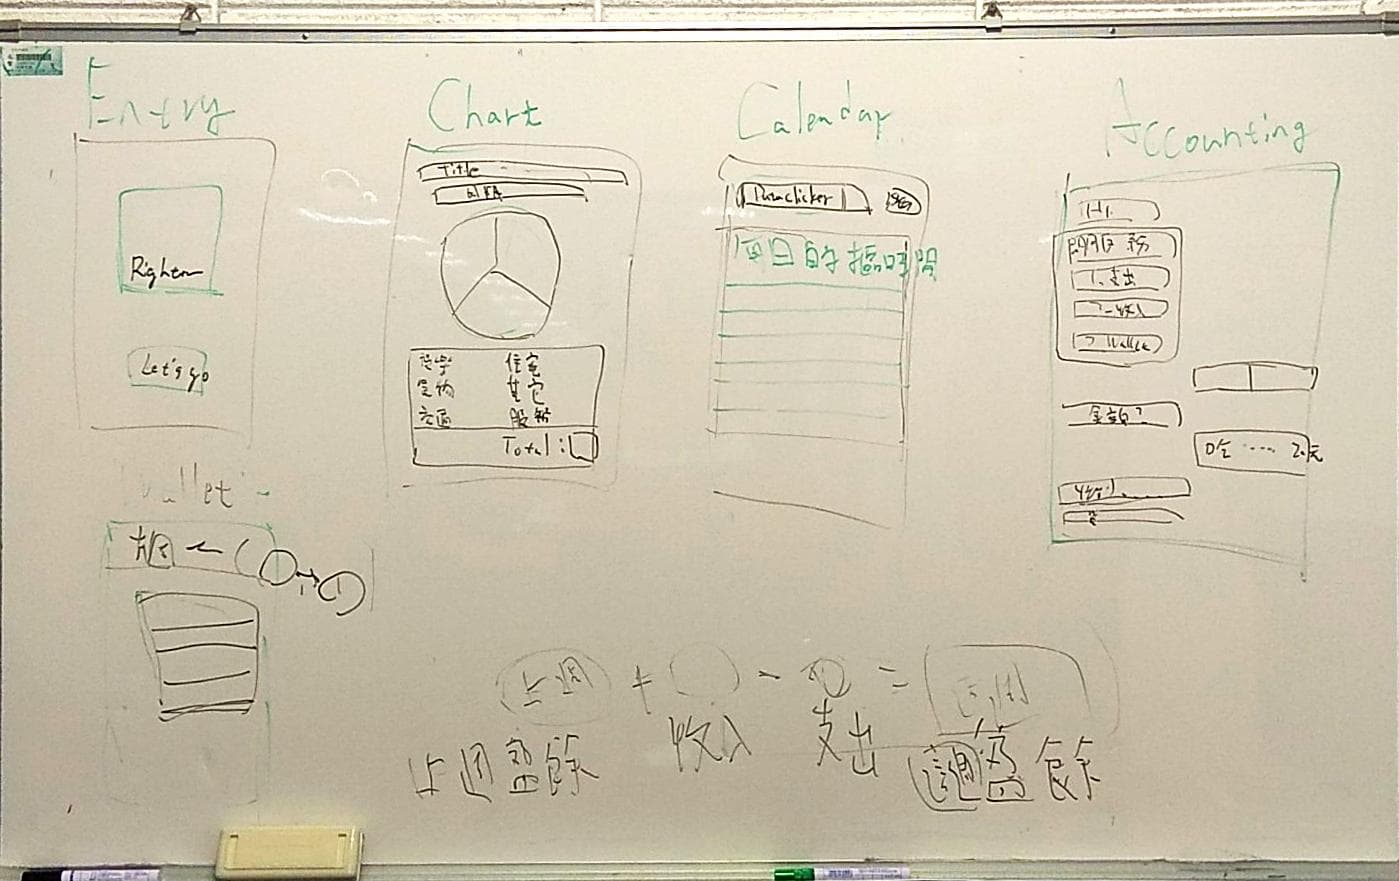
\includegraphics[width=4.75in,height=3in]{structure.jpg}\\~\\

\end{frame}

%------------------------------------------------
%------------------------------------------------

\subsection{架構圖說明} % A subsection can be created just before a set of slides with a common theme to further break down your presentation into chunks

\begin{frame}
\frametitle{功能說明}
Entry : 首頁進入畫面,點選Let's go 按鈕開啟Menu bar。\\~\\
Accounting : 進行語音記帳功能,內含新增支出、新增收入及查詢目前錢包剩餘金額。\\~\\
Chart :顯示當周花費品項分類圖表。包含住宅、娛樂、飲食、服飾、交通及其他類別。\\~\\
Calendar:查詢某日的花費。\\~\\
Wallet :顯示本周收入、支出及目前錢包剩餘金額。\\~\\

\end{frame}

%------------------------------------------------
%------------------------------------------------
\section{系統介紹} % Sections can be created in order to organize your presentation into discrete blocks, all sections and subsections are automatically printed in the table of contents as an overview of the talk
%------------------------------------------------


\subsection{系統建置環境} % A subsection can be created just before a set of slides with a common theme to further break down your presentation into chunks
\begin{frame}
\frametitle{建置環境}
UI介面: Scene builder in Gluon.\\~\\

資料庫環境: Mysql. \\~\\

編譯環境:Java jdk1.8.0-172、Run in Android 7.0(Nougat) \\~\\

開發工具: Netbeans  \\~\\

開發語言: JavaFX  \\~\\

\end{frame}

%------------------------------------------------

\subsection{頁面展示} % A subsection can be created just before a set of slides with a common theme to further break down your presentation into chunks
\begin{frame}
\frametitle{頁面展示}
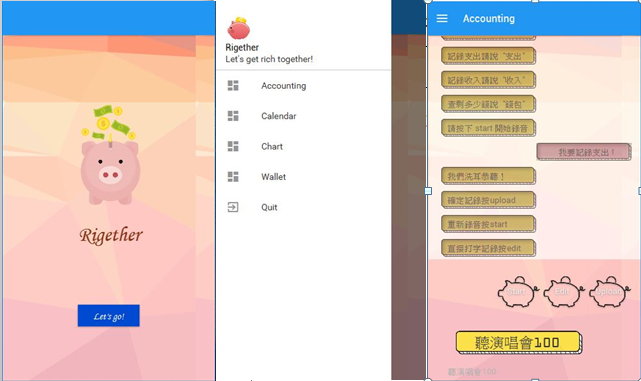
\includegraphics[width=4.75in,height=3in]{1.png}\\~\\


\end{frame}

%------------------------------------------------

\subsection{頁面展示} % A subsection can be created just before a set of slides with a common theme to further break down your presentation into chunks
\begin{frame}
\frametitle{頁面展示}
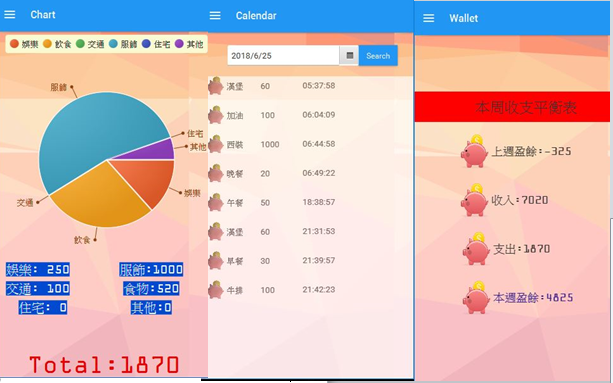
\includegraphics[width=4.75in,height=3in]{2.png}\\~\\


\end{frame}

%------------------------------------------------


\subsection{影片展示} % A subsection can be created just before a set of slides with a common theme to further break down your presentation into chunks
\begin{frame}
\frametitle{影片展示}
\href{https://www.youtube.com/watch?v=5nQ82Ot1pZI&feature=youtu.be
}{\Huge{\centerline{影片展示}}}

\end{frame}

%------------------------------------------------
\section{總結}


\subsection{參考資料} % A subsection can be created just before a set of slides with a common theme to further break down your presentation into chunks

\begin{frame}
\frametitle{參考資料}
1. Google Play : 虛擬記帳本。\\~\\~\\

2. Google Cloud Speech API : 
https://cloud.google.com/speech-to-text/?dclid=CI3I-uns89sCFdUbKgodricJ-w.\\~\\~\\


\end{frame}
%------------------------------------------------

\subsection{組員分工} % A subsection can be created just before a set of slides with a common theme to further break down your presentation into chunks

\begin{frame}
\frametitle{組員分工}
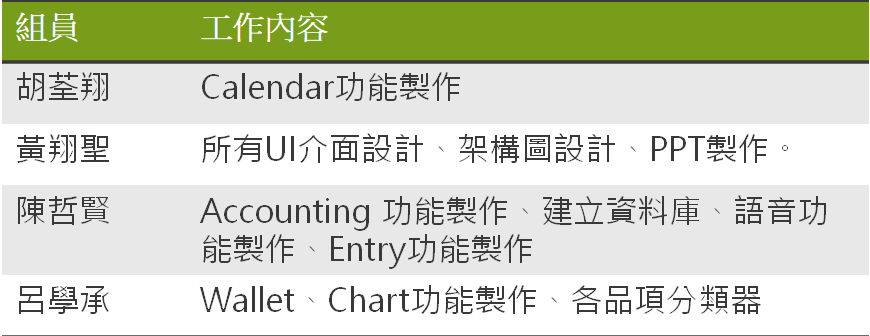
\includegraphics[width=4.75in,height=2in]{3.png}\\~\\
\end{frame}
%------------------------------------------------




\begin{frame}
\Huge{\centerline{The End}}
\end{frame}

%----------------------------------------------------------------------------------------

\end{document}